\section{Experimental Setup}
\label{sec:experimental_setup}

\subsection{Training Protocol}
\label{subsec:training}

Both the Temporal GRU and the Graph-Temporal model were trained using the
masked Pinball Loss defined in Equation~\ref{eq:masked_pinball}. Model
parameters were optimized with Adam using mini-batches of 64 samples.

Training was performed for a maximum of 200 epochs with early stopping based
on the validation Pinball Loss and a patience of 10 epochs. Whenever the
validation loss improved, the corresponding model checkpoint was retained.
Training was terminated if no further improvement was observed for 10
consecutive epochs, and the checkpoint associated with the lowest validation
loss was used for subsequent evaluation.

Both neural models use direct multi-horizon forecasting: all 12 future time
steps and the three target quantiles are predicted simultaneously from the
input history.

No test-set information was used for hyperparameter selection, early stopping,
or model calibration. The test partition was accessed only after the model
configuration had been selected using the training and validation partitions.


\subsection{Hyperparameter Selection}
\label{subsec:hyperparameters}

Hyperparameters were selected exclusively according to the validation
Pinball Loss. Separate grid searches were performed for the Temporal GRU and
the Graph-Temporal model, since the two architectures expose different
model-specific parameters. The search spaces and selected configurations are
summarized in Table~\ref{tab:hyperparameters}.

\begin{table}[t]
    \centering
    \caption{Hyperparameter search spaces and selected configurations for the
    two neural forecasting models.}
    \label{tab:hyperparameters}
    \begin{tabular}{lll}
        \toprule
        Model & Hyperparameter & Values \\
        \midrule

        Temporal GRU
        & Hidden dimension & $\{32,\mathbf{64}\}$ \\
        & GRU layers & $\{1,\mathbf{2}\}$ \\
        & Learning rate & $\{\mathbf{5\times10^{-4}},10^{-3}\}$ \\
        \midrule

        Graph-Temporal
        & Graph hidden dimension & $\{32,\mathbf{64}\}$ \\
        & GRU hidden dimension & $\mathbf{64}$ \\
        & GRU layers per block & $\{\mathbf{1},2\}$ \\
        & Learning rate & $\{\mathbf{5\times10^{-4}},10^{-3}\}$ \\
        & Diffusion depth $K$ & $\mathbf{2}$ \\
        & Graph-temporal blocks & $\mathbf{2}$ \\
        \bottomrule
    \end{tabular}
\end{table}

Selected values are highlighted in bold. The diffusion depth and number of
graph-temporal blocks were kept fixed during the main hyperparameter search;
the effect of changing the diffusion depth is investigated separately in
Section~\ref{subsec:diffusion_depth}.

For the Temporal GRU, the selected configuration uses a hidden dimension of
64, two recurrent layers, and a learning rate of $5\times10^{-4}$. The best
checkpoint was obtained at epoch 78, with a validation Pinball Loss of
0.1240.

For the Graph-Temporal model, the selected configuration uses a graph hidden
dimension of 64, a GRU hidden dimension of 64, one recurrent layer per
graph-temporal block, and a learning rate of $5\times10^{-4}$. With two
blocks and diffusion depth $K=2$, the best checkpoint was obtained at epoch
106, reaching a validation Pinball Loss of 0.1133.


The learning curves of the selected configurations are shown in
Figure~\ref{fig:learning_curves}. For both models, the training loss decreases
progressively, while the validation loss eventually reaches a minimum and
ceases to improve. The selected checkpoints therefore correspond to the
minimum validation loss rather than to the final training epoch, consistently
with the early-stopping procedure described in
Section~\ref{subsec:training}.

\begin{figure}[t]
    \centering

    \begin{subfigure}[b]{0.48\linewidth}
        \centering
        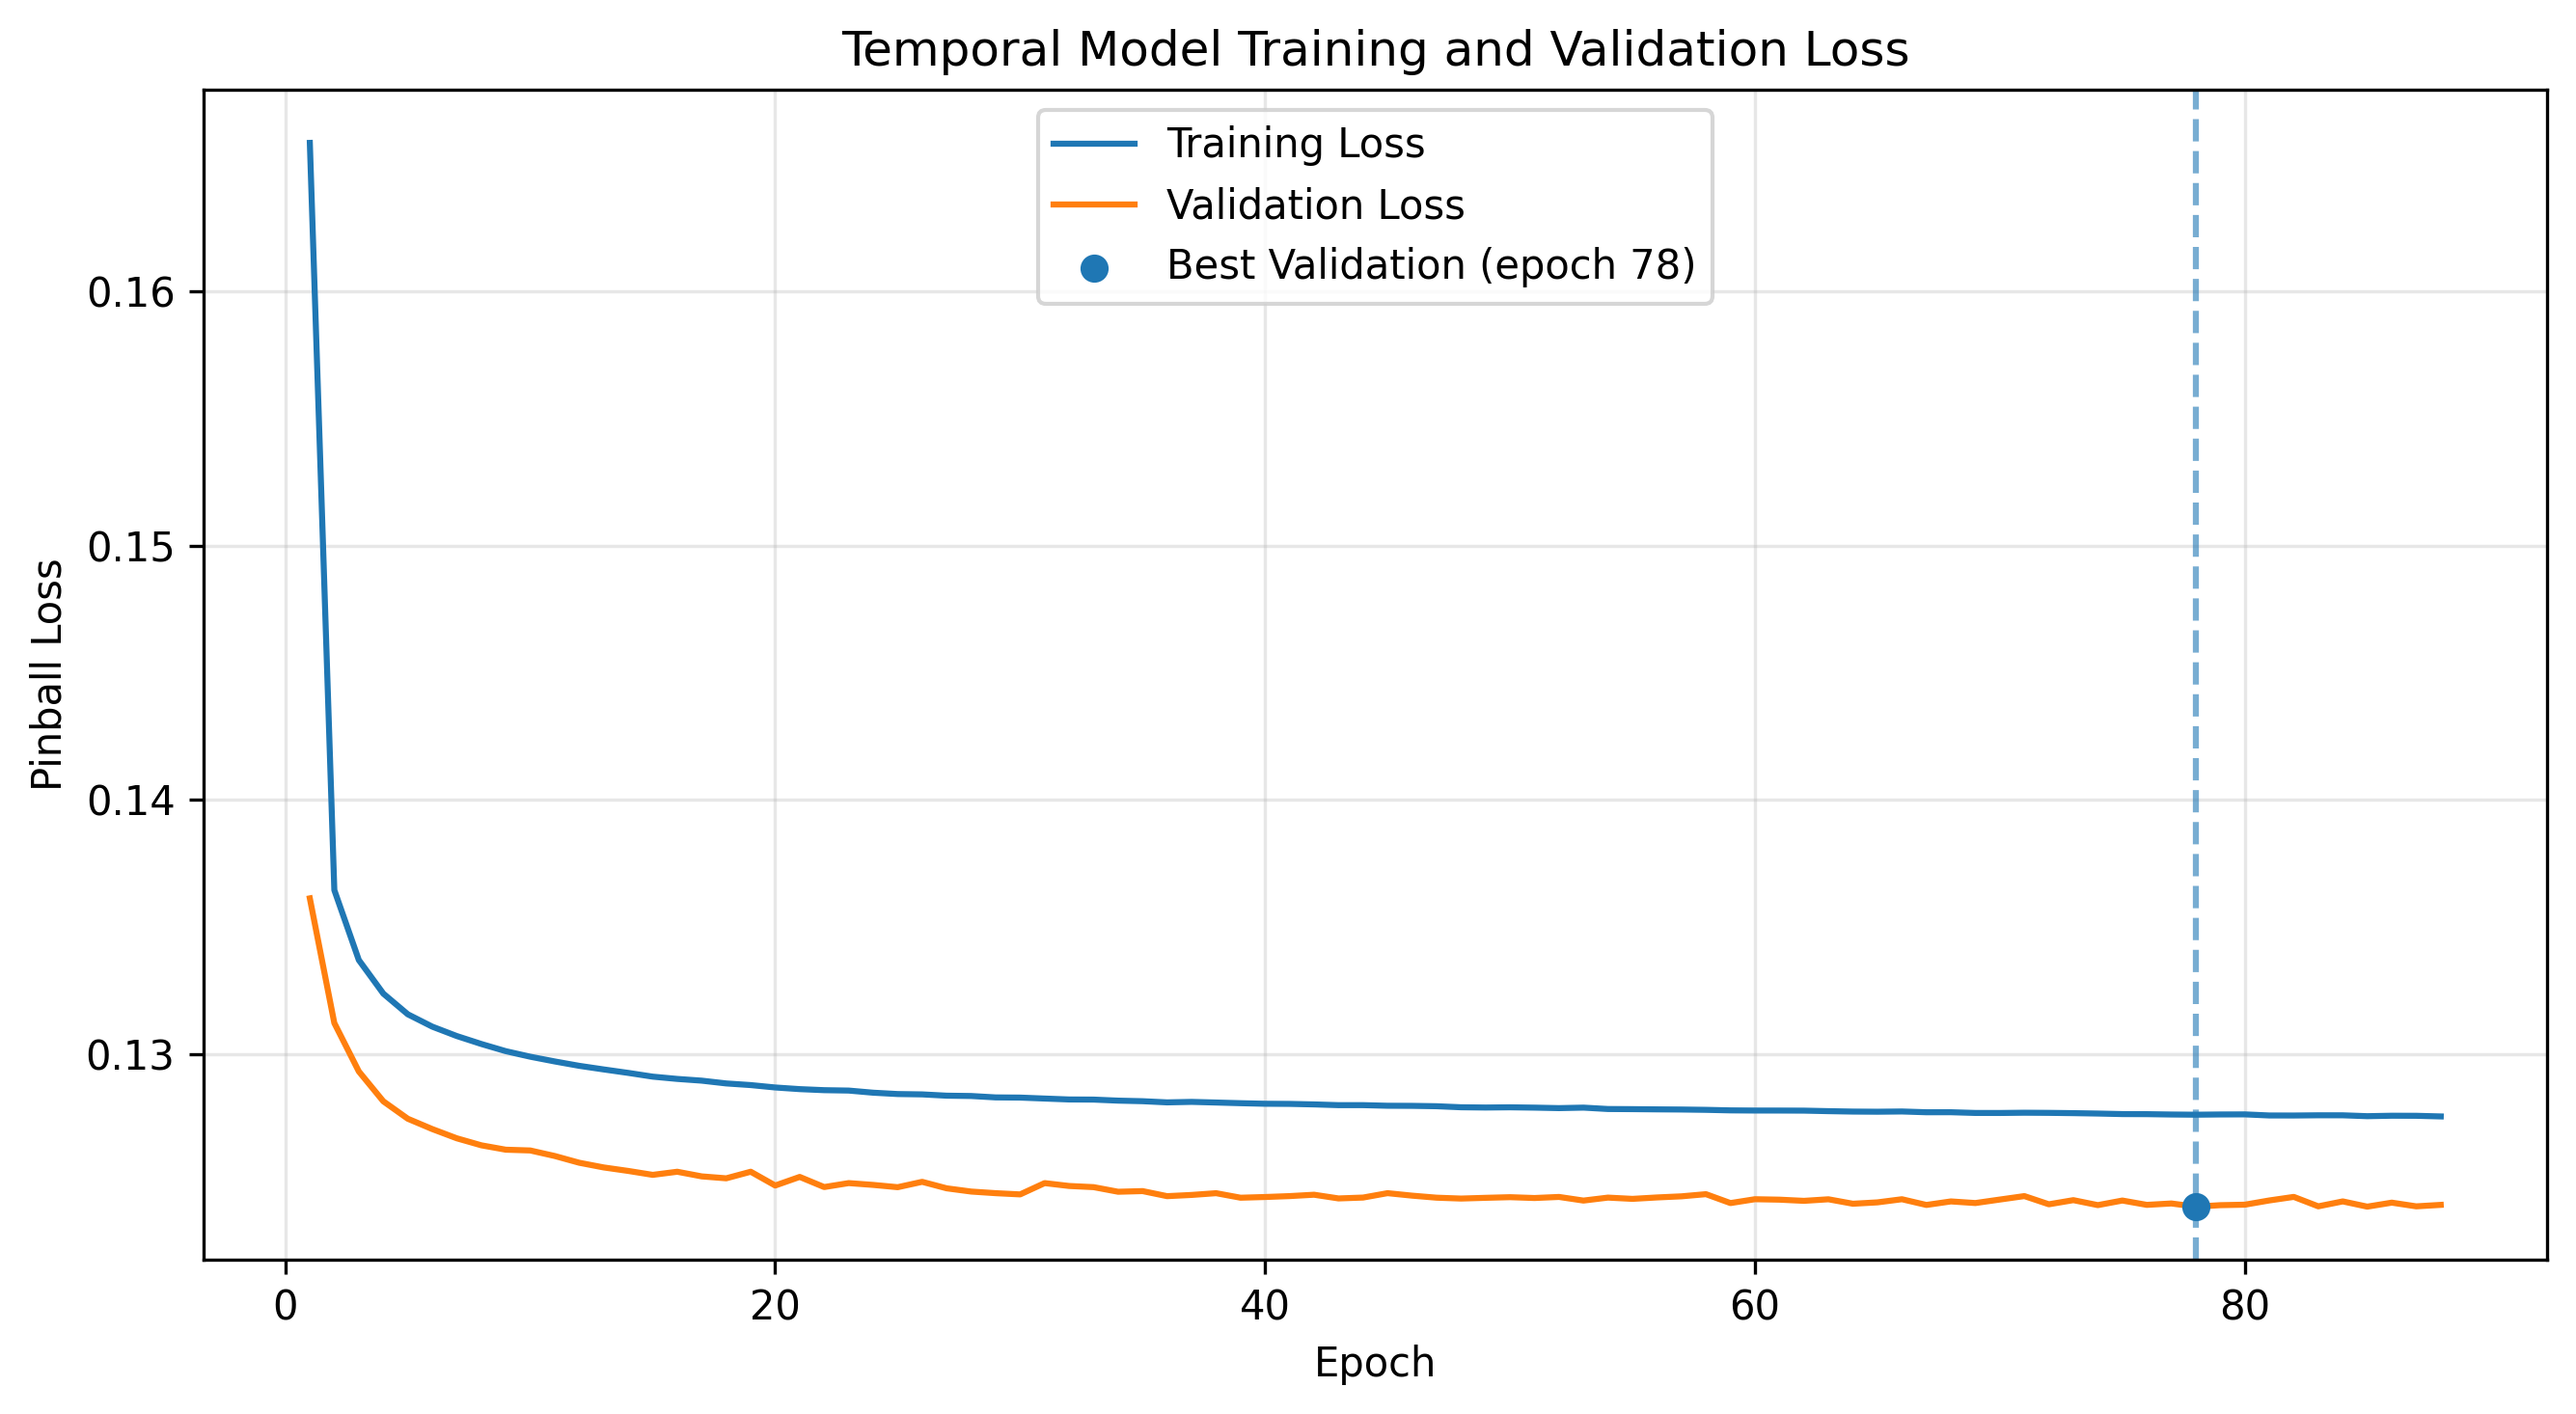
\includegraphics[width=\linewidth]{img/temporal_gru/learning_curves}
        \caption{Temporal GRU.}
        \label{fig:gru_learning_curve}
    \end{subfigure}
    \hfill
    \begin{subfigure}[b]{0.48\linewidth}
        \centering
        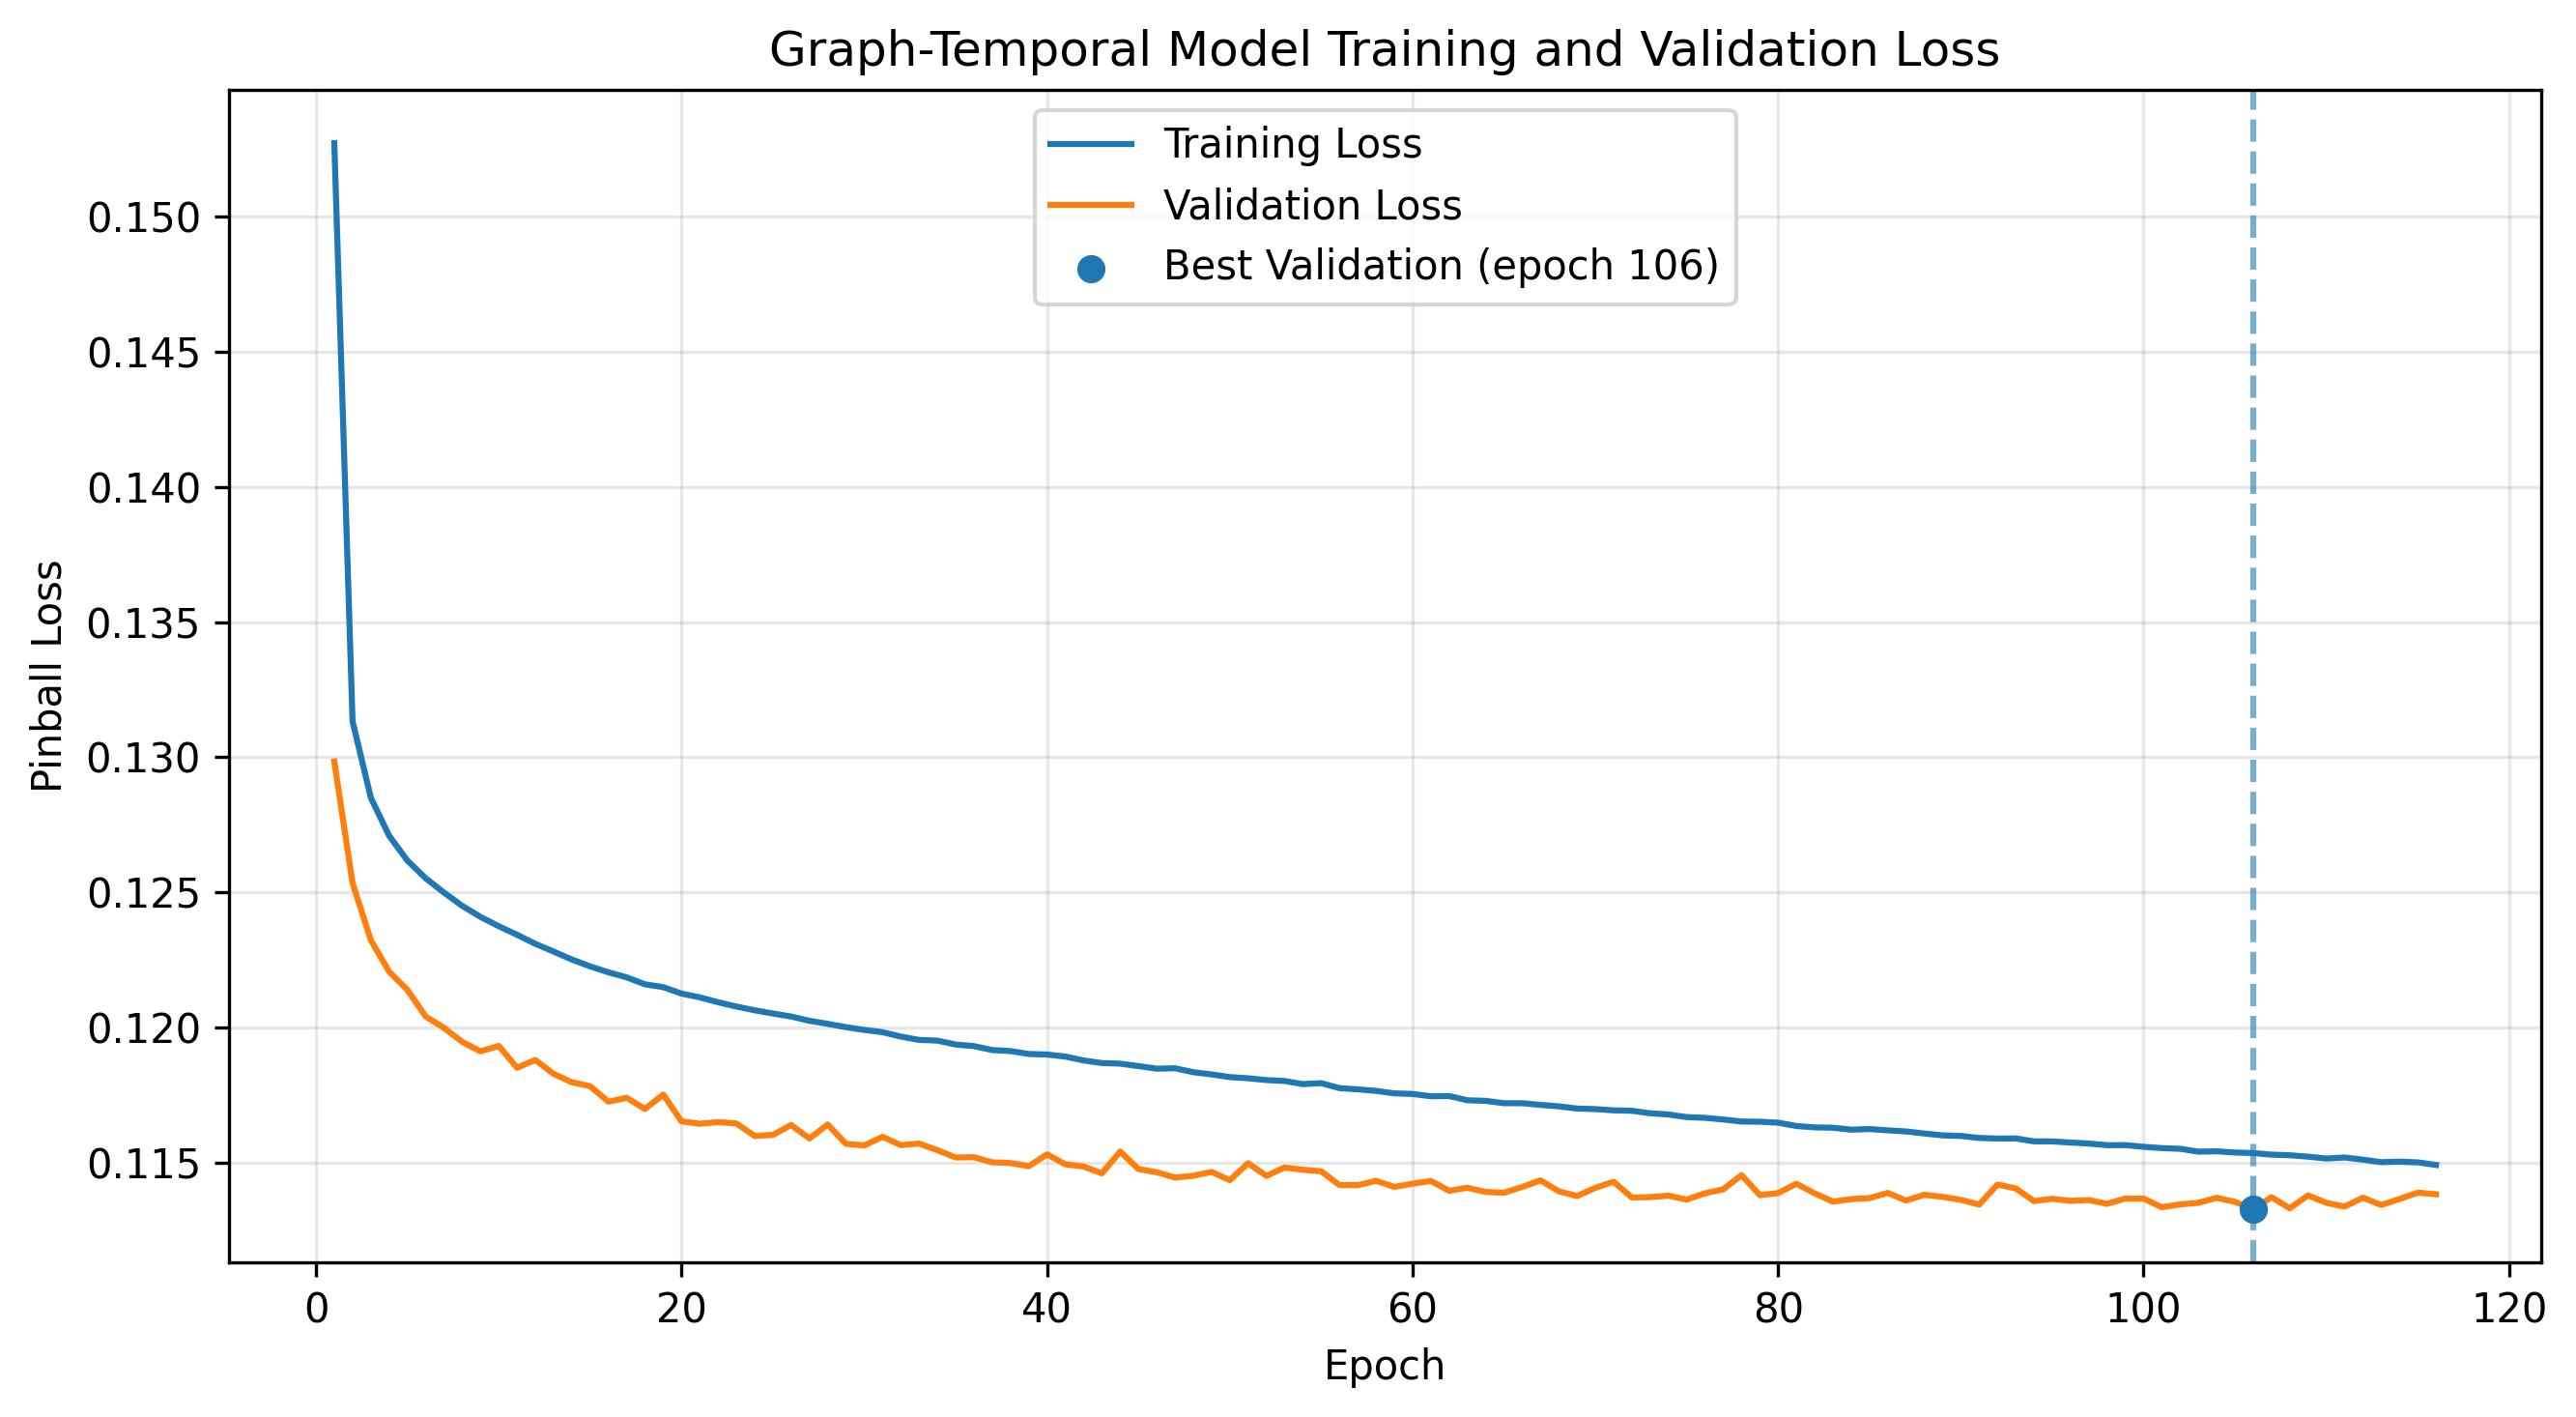
\includegraphics[width=\linewidth]{img/graph_temporal/graph_temporal_learning_curves}
        \caption{Graph-Temporal model.}
        \label{fig:graph_learning_curve}
    \end{subfigure}

    \caption{Training and validation Pinball Loss for the selected model
    configurations.}
    \label{fig:learning_curves}
\end{figure}

Validation Pinball Loss was used as the single model-selection criterion
rather than selecting configurations directly according to empirical
coverage. This criterion evaluates the quality of the predicted quantiles
without optimizing the model specifically for a single coverage statistic.
Coverage and interval width were instead retained as complementary
reliability metrics for the final analysis.


\subsection{Evaluation Metrics}
\label{subsec:metrics}

Performance is evaluated at the three forecasting horizons of 15, 30, and 60 minutes. All metrics are
computed only over valid target observations using the corresponding target
availability mask.

Point forecasting accuracy is evaluated using the median prediction
$\hat{y}^{(0.5)}$. The Mean Absolute Error (MAE) is defined as

\begin{equation}
    \mathrm{MAE}
    =
    \frac{1}{|\Omega|}
    \sum_{i\in\Omega}
    \left|
        y_i-\hat{y}^{(0.5)}_i
    \right|,
    \label{eq:mae}
\end{equation}

where $\Omega$ denotes the set of valid target entries at the considered
forecast horizon.

The Root Mean Squared Error (RMSE) is defined as

\begin{equation}
    \mathrm{RMSE}
    =
    \sqrt{
        \frac{1}{|\Omega|}
        \sum_{i\in\Omega}
        \left(
            y_i-\hat{y}^{(0.5)}_i
        \right)^2
    }.
    \label{eq:rmse}
\end{equation}

While MAE measures the average magnitude of the forecasting error, RMSE
assigns greater weight to large deviations and is therefore useful for
identifying models that occasionally produce particularly inaccurate
forecasts.

Probabilistic forecasting quality is evaluated through the Pinball Loss
introduced in Equation~\ref{eq:pinball_loss}. The loss is reported
separately for $q_{0.1}$, $q_{0.5}$, and $q_{0.9}$, allowing the quality of
the lower, median, and upper conditional quantile estimates to be examined
individually.

The reliability of the predictive intervals is assessed through empirical
coverage. For the nominal 80\% interval
$[\hat{y}^{(0.1)},\hat{y}^{(0.9)}]$, coverage is computed as

\begin{equation}
    \mathrm{Coverage}
    =
    \frac{1}{|\Omega|}
    \sum_{i\in\Omega}
    \mathbb{I}
    \left[
        \hat{y}^{(0.1)}_i
        \leq y_i
        \leq
        \hat{y}^{(0.9)}_i
    \right],
    \label{eq:coverage}
\end{equation}

where $\mathbb{I}[\cdot]$ is the indicator function. A well-calibrated
80\% predictive interval is expected to contain approximately 80\% of the
observed targets.

Coverage alone is not sufficient to characterize forecast quality, since
arbitrarily wide intervals could achieve high coverage. Predictive sharpness
is therefore evaluated using the mean interval width,

\begin{equation}
    \mathrm{Width}
    =
    \frac{1}{|\Omega|}
    \sum_{i\in\Omega}
    \left(
        \hat{y}^{(0.9)}_i
        -
        \hat{y}^{(0.1)}_i
    \right).
    \label{eq:interval_width}
\end{equation}

Coverage and interval width are interpreted jointly: reliable forecasts
should achieve coverage close to the nominal level while keeping predictive
intervals as informative as possible.

Finally, the quantile crossing rate measures the fraction of predictions for
which the estimated quantiles violate their expected ordering,

\begin{equation}
    \hat{y}^{(0.1)}
    \leq
    \hat{y}^{(0.5)}
    \leq
    \hat{y}^{(0.9)}.
\end{equation}

A crossing rate close to zero indicates that the independently predicted
quantiles are almost always ordered consistently.

In addition to these scalar metrics, calibration plots are used to compare
the nominal quantile levels with their empirical frequencies. This provides
a more detailed view of probabilistic calibration than the 80\% interval
coverage alone.


\subsection{Hardware and Reproducibility}
\label{subsec:hardware}

All neural models were implemented in PyTorch and trained using an NVIDIA
GeForce RTX 4060 Laptop GPU with CUDA acceleration. A fixed random seed of
42 was used throughout the experiments to improve reproducibility.

Model checkpoints corresponding to the best validation Pinball Loss were
saved during training and subsequently reloaded for final evaluation. The
same preprocessing pipeline, dataset partitions, forecast horizons, and
evaluation functions were used across the learned models to ensure a
consistent experimental comparison.